\section{Discussion}
\chapter{Discussion}
\section{Further development}
Not all the intended functionality got added to the map. This section will list some of the features, which there was not time to implement. 

\subsection{Data at point of click}

A function could be added to get the population counts from a clicked point for both maps. An example of this have been shown in figure x. When the user clicks the map an infobox informs the user about the value at the clicked point for both maps. 
TODO: Figure showing a popup on click
-	Popup text: Data in this map and data in the other



\subsection{Parallel generation of tiles}
As mentioned in section x the generation of tiles were done without using multiple processers, which meant that it became a time-consuming process. With the official gdal2tiles being able to generate tiles following the XYZ standard it is possible that using this would allow for parallel generation of tiles. 
This is probably the most important missing feature, since the processing time otherwise would be so high, that it would not be a faster alternative to the currently available options. 

\subsection{Changing layers}
Another functionality, which could have been added was the option to change the datasets of the maps. As mentioned in section x the case data contains population projection for ten different years. It does therefore make sense to have the option display more than the two datasets.  As illustrated in figure x data from other years could be added as separate layers. This would allow the user to compare different datasets without having to reload the webgis with different datasets.

This way the map could also be used to visualize the different in the same projection from one year and another.
\subsection{Option for multiple colorschemes}
If there is a vast difference between the values in the two shown projection coloring based on the same maximum values does not necessarily make sense as was shown in the figure in core concept 2. It would therefore make sense to have the option to enable separate coloring as shown in figure x. 
TODO: make a figure showing the map with multiple legends and color schemes. 


\section{Performance enhancements}

Based on the performance and best practice audits by Google Lighthouse the performance could be enhanced in multiple ways. 

\textbf{Eliminate render-blocking resources}
As mentioned in section x the largest render-blocking resource was Openlayers. The same section also highlighted that 43.2 \% of the library never get used. The performance could therefore be improved by only loading the necessary parts of the library. 
\fxnote{Check with Carsten – can this only be done with node?}
https://openlayers.org/en/latest/doc/tutorials/bundle.html

\textbf{Avoid enormous network payloads}
The size of data loads will be reduced by only having to load one set of tiles with the solution mentioned in section x. 

\fxnote{Write about asynchronous XMLREquest and minifying/compressing}
-	Tenser 

\fxnote{Write about zoom level bug}
\fxnote{Add user testing to future work }

\textbf{Does not use HTTP/2 for all of its resources}
Caddy was used to serve the resources with HTTP/2. However even after setting up Caddy the error message was still present. It is uncertain if this means that the connection still is HTTP/1 based or if it is HTTP/2 but labelled incorrectly. Figure x is two screenshots from the network tab of chromes developer tool when the page is served with a python server (top) and caddy server (bottom). 
The grey bars are when a loaded file is being stalled. The blue bars are when they are loaded. This figure shows that the serving is being optimized, where the stalling largely is gone. This could indicate that the server no longer has the HTTP/1 limit of only having 6 TCP connections.
 

\begin{figure} [H]
	\centering
	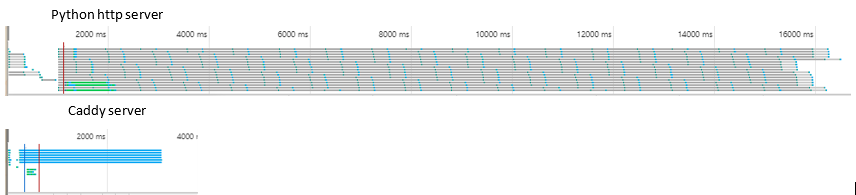
\includegraphics[width=.8\textwidth]{Pictures/CaddyVsPython}
	\caption{Screenshot of the network connection for a python and a caddy server}
	\label{CaddyVsPython}
\end{figure}


\fxnote{Mention caddy – 6 connection issue earlier}
 

\section{Is this even a good measurement for performance?}
